\documentclass[11pt, a4paper]{article}

\usepackage{amsmath}
\usepackage{amsfonts} %Matheschriften
\usepackage{amssymb} %Mathesymbole
%\usepackage{mathptmx} % Einstellung für Schriften und Sonderzeichen in mathematischen Umgebungen
                        % ändert SChriftfont
\usepackage{wasysym} % Stellt diverse Sonderzeichen bereit
\usepackage{siunitx}
\usepackage{float}
\usepackage{microtype}
\usepackage{graphicx}
\usepackage{hyperref}
\usepackage{xcolor}
\usepackage[section]{placeins}
% allows for temporary adjustment of side margins
\usepackage{changepage}
\usepackage{rotating}
\usepackage{tikz}
\usetikzlibrary{calc}


\usepackage[ngerman]{babel}
\addto\captionsngerman{%
 \renewcommand{\abstractname}{Einleitung}}

\title{Versuch 4: Optik}
\author{Team 4-11: Jascha Fricker, Benedict Brouwer}

\begin{document}
    \maketitle

    \tableofcontents

    \newpage

    \section{Einleitung}
    In der Physik spielen Linsen in optischen Versuchsuafbauten eine sehr wichtige Rolle. In diesem Versuch soll es darum gehen, verschiedene 
    Methoden auszuprobieren um den Brechungsindex und Hauptebenenabstand verschiedener Lisnen bzw Linsensysteme zu messen.

    \section{Theorie}

    \subsection{Dünne Linsen}
    \paragraph{Autokollimationsmethode}
    Bei Autokollimationsmethode ist die Brennweite
    \begin{align}
        f = d \label{eq:auto}
    \end{align}
    bei dünnen Linsen genau der Abstand $d$ zwischen Objekt/Bild und Linse.
    \paragraph{Besselmethode}
    Bei der Besselmethode kann die Brennweite
    \begin{align}
        f = \frac{1}{4} \left( e - \frac{d^2}{e} \right) = \frac{1}{4} \left( e - \frac{\left(a_2 - a_1\right)^2}{e} \right) \label{eq:bessel}
    \end{align}
    durch die zwei Positionen der Linse $a_1$ und $a_2$ und den Abstand Objekt-Schirm $e$ bestimmt werden.
    
    \subsection{Optisches System}

    Für die Gesamtbrennweite und Hauptebenen eines Optischen Systems gilt
    \begin{align}
        f &= \frac{f_1' \cdot f_2'}{t - f_1' - f_2'} \label{eq:brenn}\\
        h &= \frac{f_1}{f_1 + f_2 + f_3 + \dots} \label{eq:ebene}
    \end{align}

    \paragraph*{Bessel- und Autokollimationsmethode}
    Bei dicken Linsen kann durch zusammenführen der Besselmethode und Autokollimationsmethode die Brennweite $f'$ und der Hauptebenenabstand $h$
    
    \begin{align} \begin{split} \label{eq:dicke}
        f' &= \frac{1}{2} \sqrt{(e-k-l)^2 - d^2} \\
        h &= k + l - \sqrt{(e-k-l)^2 - d^2} \end{split}
    \end{align}
        
    bestimmt werden. Dabei ist $d = a_2 - a_1$ die Distanz zwischen den beiden Positionen der Linse, $e$ der Abstand zwischen Objekt und Schirm, $k$ der Abstand zwischen Linse und Objekt/Bild und $l$ der Abstand zwischen Objekt/Bild bei umgedrehten Linsensystem.

    \paragraph{Messmethode nach Abbe}
    Es gelten die zwei Beziehungen
    \begin{align}
        g &= f \cdot \left(1 - \frac{1}{\beta}\right) + h_1 \label{eq:dicke1} \\
        g' &= f' \cdot (1 - \beta) + h_2 \label{eq:dicke2} \\
        \text(mit) \ \ \beta = \frac{y'}{y}
    \end{align}
    Durch fitten an die Daten für den Abstand zum Objekt $g$ bzw zum Bild $g'$ kann die Brennweite $f$ bzw $f'$ und der Hauptebenenabstand $h_1$ und $h_2$ bestimmt werden.


    \section{Ergebnisse}
    \subsection{Aufgabe 1}
    Als erstes wurden alle Linsen angeschaut. Durch beobachten des Millimeterpapiers durch die Linsen konnte zwischen einem vergrößernden Effekt (Konvexe Linse) und einem verkleinerndem Effekt (Konkave Linse) unterschieden werden. Nur die Linse E konnte als Streulise identifiziert werden, alle anderen Linsen waren als Sammellisen zu erkennen.

    \subsection{Einzellinsen}
    Die Ergebnisse der Autokollimationsmethode und der Besselmethode sowie der gewichtete Mittelwert der beiden Methoden wurden mit den Formel (\ref{eq:auto}) und (\ref{eq:bessel}) sind in der Tabelle \ref{tab:ergebnisse} dargestellt.

    \begin{table}[h]
        \centering
        \begin{tabular}{c|c|c}
            Methode & Brennweite B & Brennweite G \\ \hline
            Autokollimation & $10,04(5) \si{\centi\metre}$ & $7,49(7) \si{\centi\metre}$ \\ \hline
            Bessel & $9,97(8) \si{\centi\metre}$ & $7,488(35) \si{\centi\metre}$ \\ \hline
            Mittelwert & $10.02(4) \si{\centi\metre}$ & $7.492(31) \si{\centi\metre}$
        \end{tabular}
        \caption{Brennweiten der Linsen B und G}
        \label{tab:ergebnisse}
    \end{table}
    Der Fehler der Länge wurde mit Tabelle 5 des ABW-Skripts \cite{ABW} berechnet und durch den gewichteten Mittelwert fortgepflanzt.

    \subsection{Linsensystem}
    Wir haben das Linsensystem E-G mit $30$ mm Abstand für unsere Messungen benutzt.

    \paragraph{Autokollimation- und Besselmethode}
    Mit Gleichung \ref{eq:dicke} konnte aus den Messwerten der beiden Methoden die Brennweite und der Hauptebenenabstand
    \begin{align}
        f' &= 13,10(20) \si{\centi\metre} \\
        h &= 0,3(6) \si{\centi\metre}
    \end{align}
    bestimmt werden. Der Fehler der Länge wurde mit Tabelle 5 des ABW-Skripts \cite{ABW} berechnet und der gewichtete Mittelwert wurde genutzt.

    \paragraph{Messmethode nach Abbe}
    Um die Brennweiten und Hauptebenenabstände zu bestimmen,
    \begin{align}
        f &= 14,21(28) \si{\centi\metre} \\
        f' &= -12,74(19) \si{\centi\metre} \\
        h_1 &= -21,62(43) \si{\centi\metre} \\
        h_2 &= 32,31(59) \si{\centi\metre}
    \end{align}
    
    wurden die Messwerte für den Abstand zum Objekt $g$ und zum Bild $g'$ mit den Formeln (\ref{eq:dicke1}) und (\ref{eq:dicke2}) gefittet. Die Fits sind in \ref{fig:fit1} und \ref{fig:fit2} dargestellt.

    \begin{figure}[h]
        \centering
        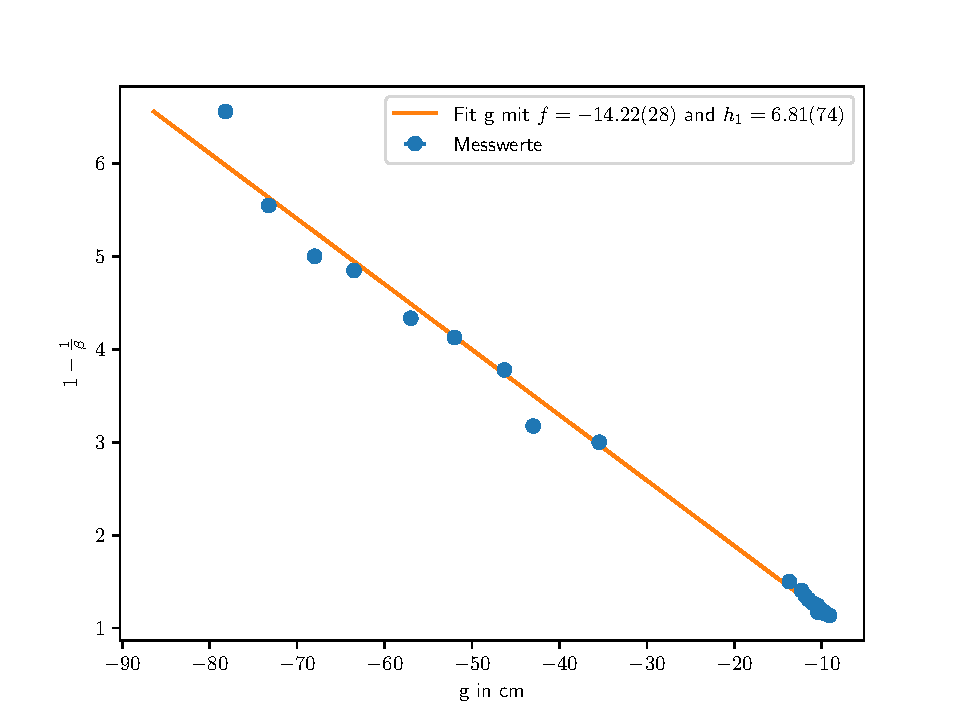
\includegraphics[width=0.8\textwidth]{g.pdf}
        \caption{Fit der Messwerte für den Abstand zum Objekt}
        \label{fig:fit1}
    \end{figure}

    \begin{figure}[h]
        \centering
        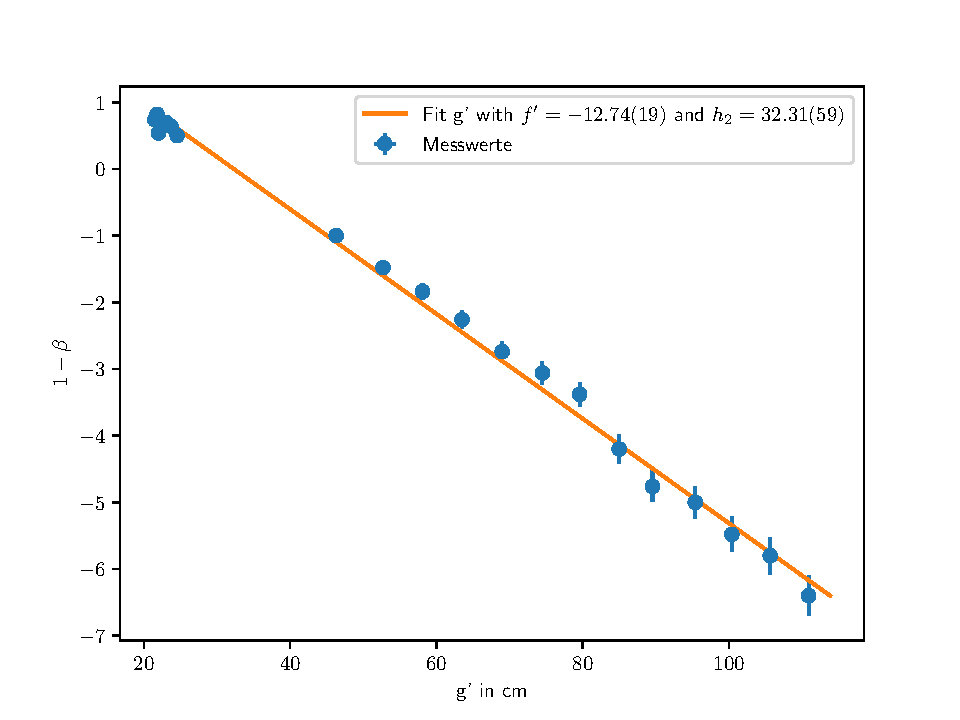
\includegraphics[width=0.8\textwidth]{g_prime.pdf}
        \caption{Fit der Messwerte für den Abstand zum Bild}
        \label{fig:fit2}
    \end{figure}

    % Bild des Aufbaus


    \begin{figure}[h]
        \centering
        \begin{tikzpicture}[scale=0.2]
            % Define lens properties
            \def\lensRadius{10}
            \def\lensHeight{12}
            \def\lensWidth{1}
            \def\focalLengthOne{-5} % concave lens
            \def\focalLengthTwo{5} % convex lens
            \def\startAngle{asin(\lensHeight/\lensRadius)}
            \pgfmathsetmacro{\lensRadius}{50}
            \pgfmathsetmacro{\lensHeight}{10}
            \pgfmathsetmacro{\startAngle}{asin(\lensHeight/\lensRadius)}


            % Draw lenses
            \draw [fill=blue!15]  (3,\lensHeight)
            arc[start angle=180-\startAngle,delta angle=2*\startAngle,radius=\lensRadius]
            arc[start angle=-\startAngle,delta angle=2*\startAngle,radius=\lensRadius]
             -- cycle; % to get a better line end
            \draw [fill=blue!15] (\lensWidth,\lensHeight)
            arc[start angle=180-\startAngle,delta angle=2*\startAngle,radius=\lensRadius] -- (-\lensWidth, -\lensHeight)
            arc[start angle=-\startAngle,delta angle=2*\startAngle,radius=\lensRadius]
             -- cycle; % to get a better line end
            % Draw principal planes
            \draw [dashed] (-21.629, -1*\lensHeight) -- (-21.629, 1*\lensHeight);
            \draw [dashed] (32.309, -1*\lensHeight) -- (32.309, 1*\lensHeight);

            % Draw focal points
            \filldraw (14.217 - 21.629,0) circle (4pt);
            \filldraw (-12.741 + 32.30 ,0) circle (4pt);

            % Label lenses
            \node at (-3,-8) {Concave};
            \node at (13,-8) {Convex};

            % Label principal planes and focal points
            \node at (-21.629,-14) {$P_1$};
            \node at (14.217 - 21.629,-14) {$F_1$};
            \node at (32.309,-14) {$P_2$};
            \node at (-12.741 + 32.30 ,-14) {$F_2$};

            % Draw optical axis
            \draw [->](-25,0)--(40,0);

            % Label optical axis
            %\node at(30,-3){Optical Axis};

        \end{tikzpicture}
        \caption{Bild des Aufbaus}
        \label{fig:aufbau}
    \end{figure}


    \subsubsection{Berechnung der Brennweiten und Hauptebenen}
    Durch umstellen der Gleichung (\ref{eq:brenn}) nach $f_E$ kann die Brennweite der ersten Linse E bei durch Aufgaben 2 und 3 gegebener Brennweite $f_G = 7.492(31) \si{\centi\metre}$ und $f' = - 13,10(20) \si{\centi\metre}$ berechnet werden. Der Abstand $t = 3 \si{\centi\metre}$ ist auch gegeben.

    \begin{align}
        f_E = \frac{f' \left(t - f'\right)}{f' - f_G} = 10.24(20) \si{\centi\metre}
    \end{align}

    Diese Wert für $f_E$ stimmt sehr gut mit der Vorgabe überein, hat aber nur eine kleine Unsicherheit.






    \section{Diskussion}

    \bibliographystyle{plain}
    \bibliography{literature}

\end{document}